\documentclass[notitlepage,12pt]{article}
\usepackage[margin=1in]{geometry}
\usepackage{natbib}
\usepackage{graphicx}
\usepackage{titling}
\usepackage{url}
\graphicspath{{../img}}

% base word count 27
\title{%
MAIGG Water Bottle in Renderman  \\
\large Rendering Assignment}
\author{}
\date{12/05/2021}

\begin{document}
\maketitle

% \thispagestyle{empty}

% \begin{abstract}
% \noindent TODO
% \end{abstract}

% \newpage
% \clearpage
% \setcounter{page}{1}

\section{Analysis and Implementation}

% one paragraph for each analysing the reference images for the following points
% one paragraph for each analysing the implementation

\subsection{The Model} \label{section:model}

\begin{figure}[ht]
    \centering
    \begin{minipage}[b]{0.3\textwidth}
        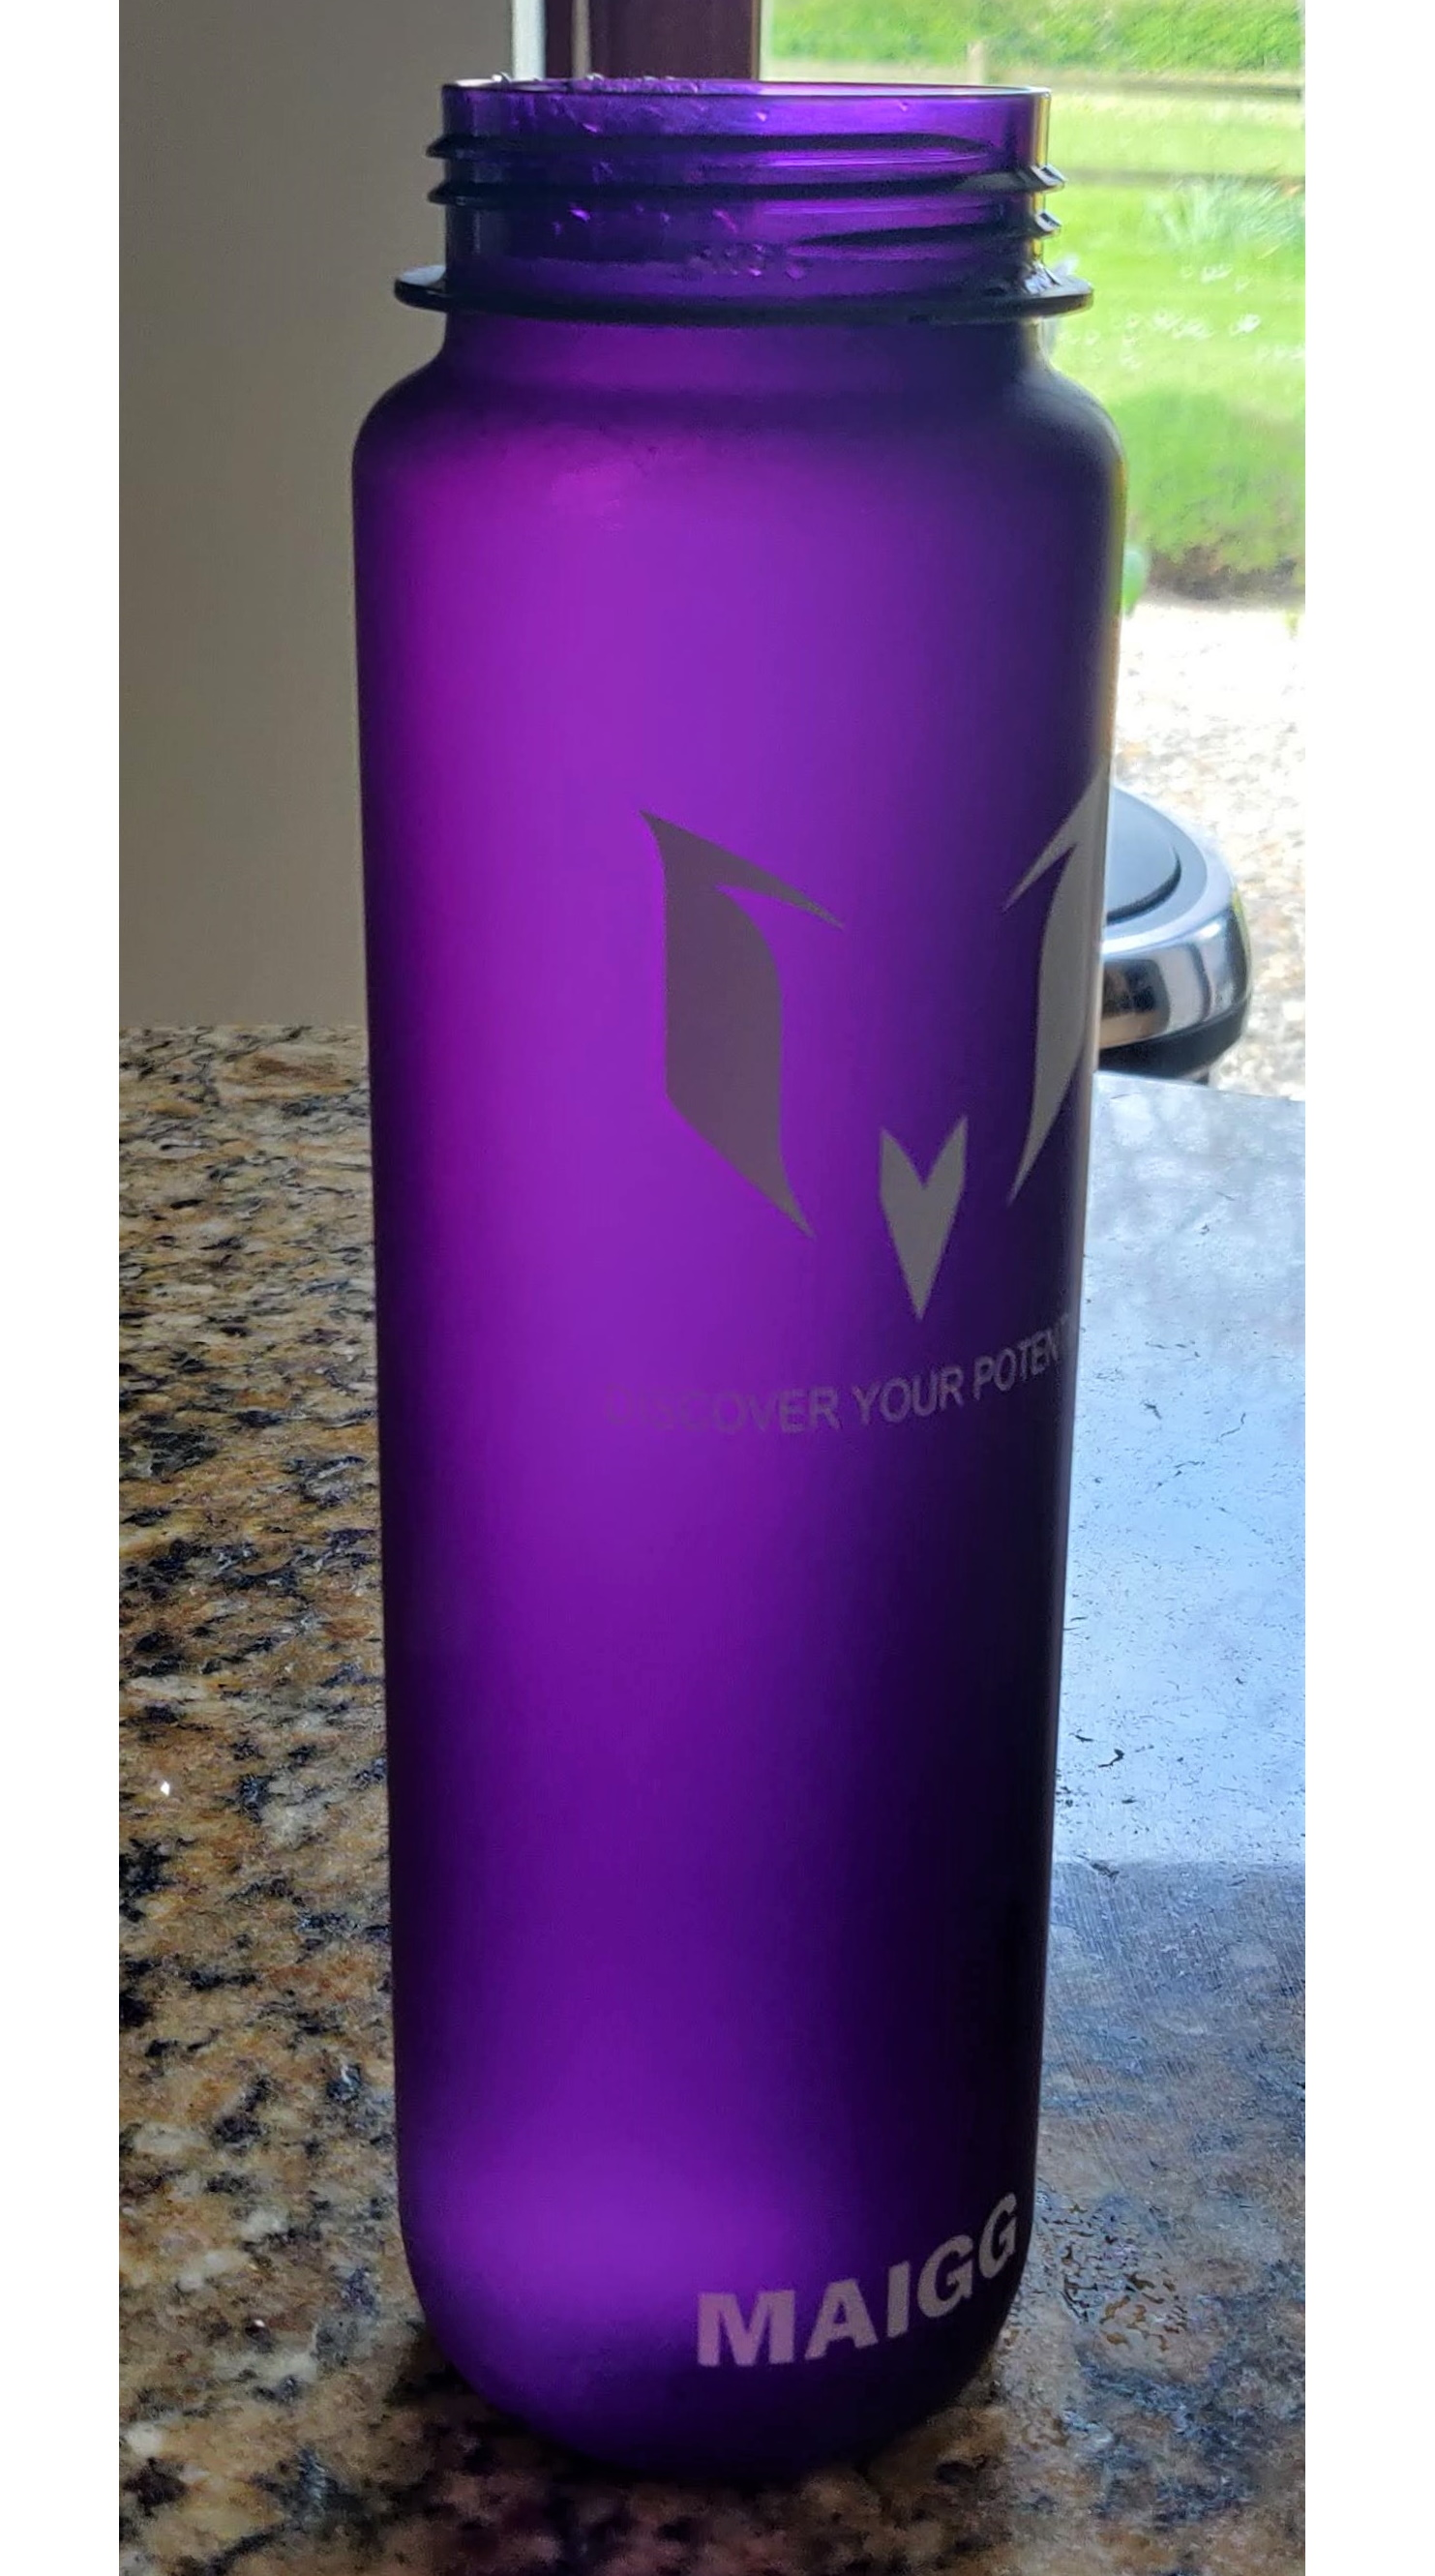
\includegraphics[width=\textwidth]{reference/bottle_left.jpg}
        \caption{Left side of bottle with back light showing slight transparency.}
        \label{fig:left}
    \end{minipage}
    \hfill
    \begin{minipage}[b]{0.3\textwidth}
        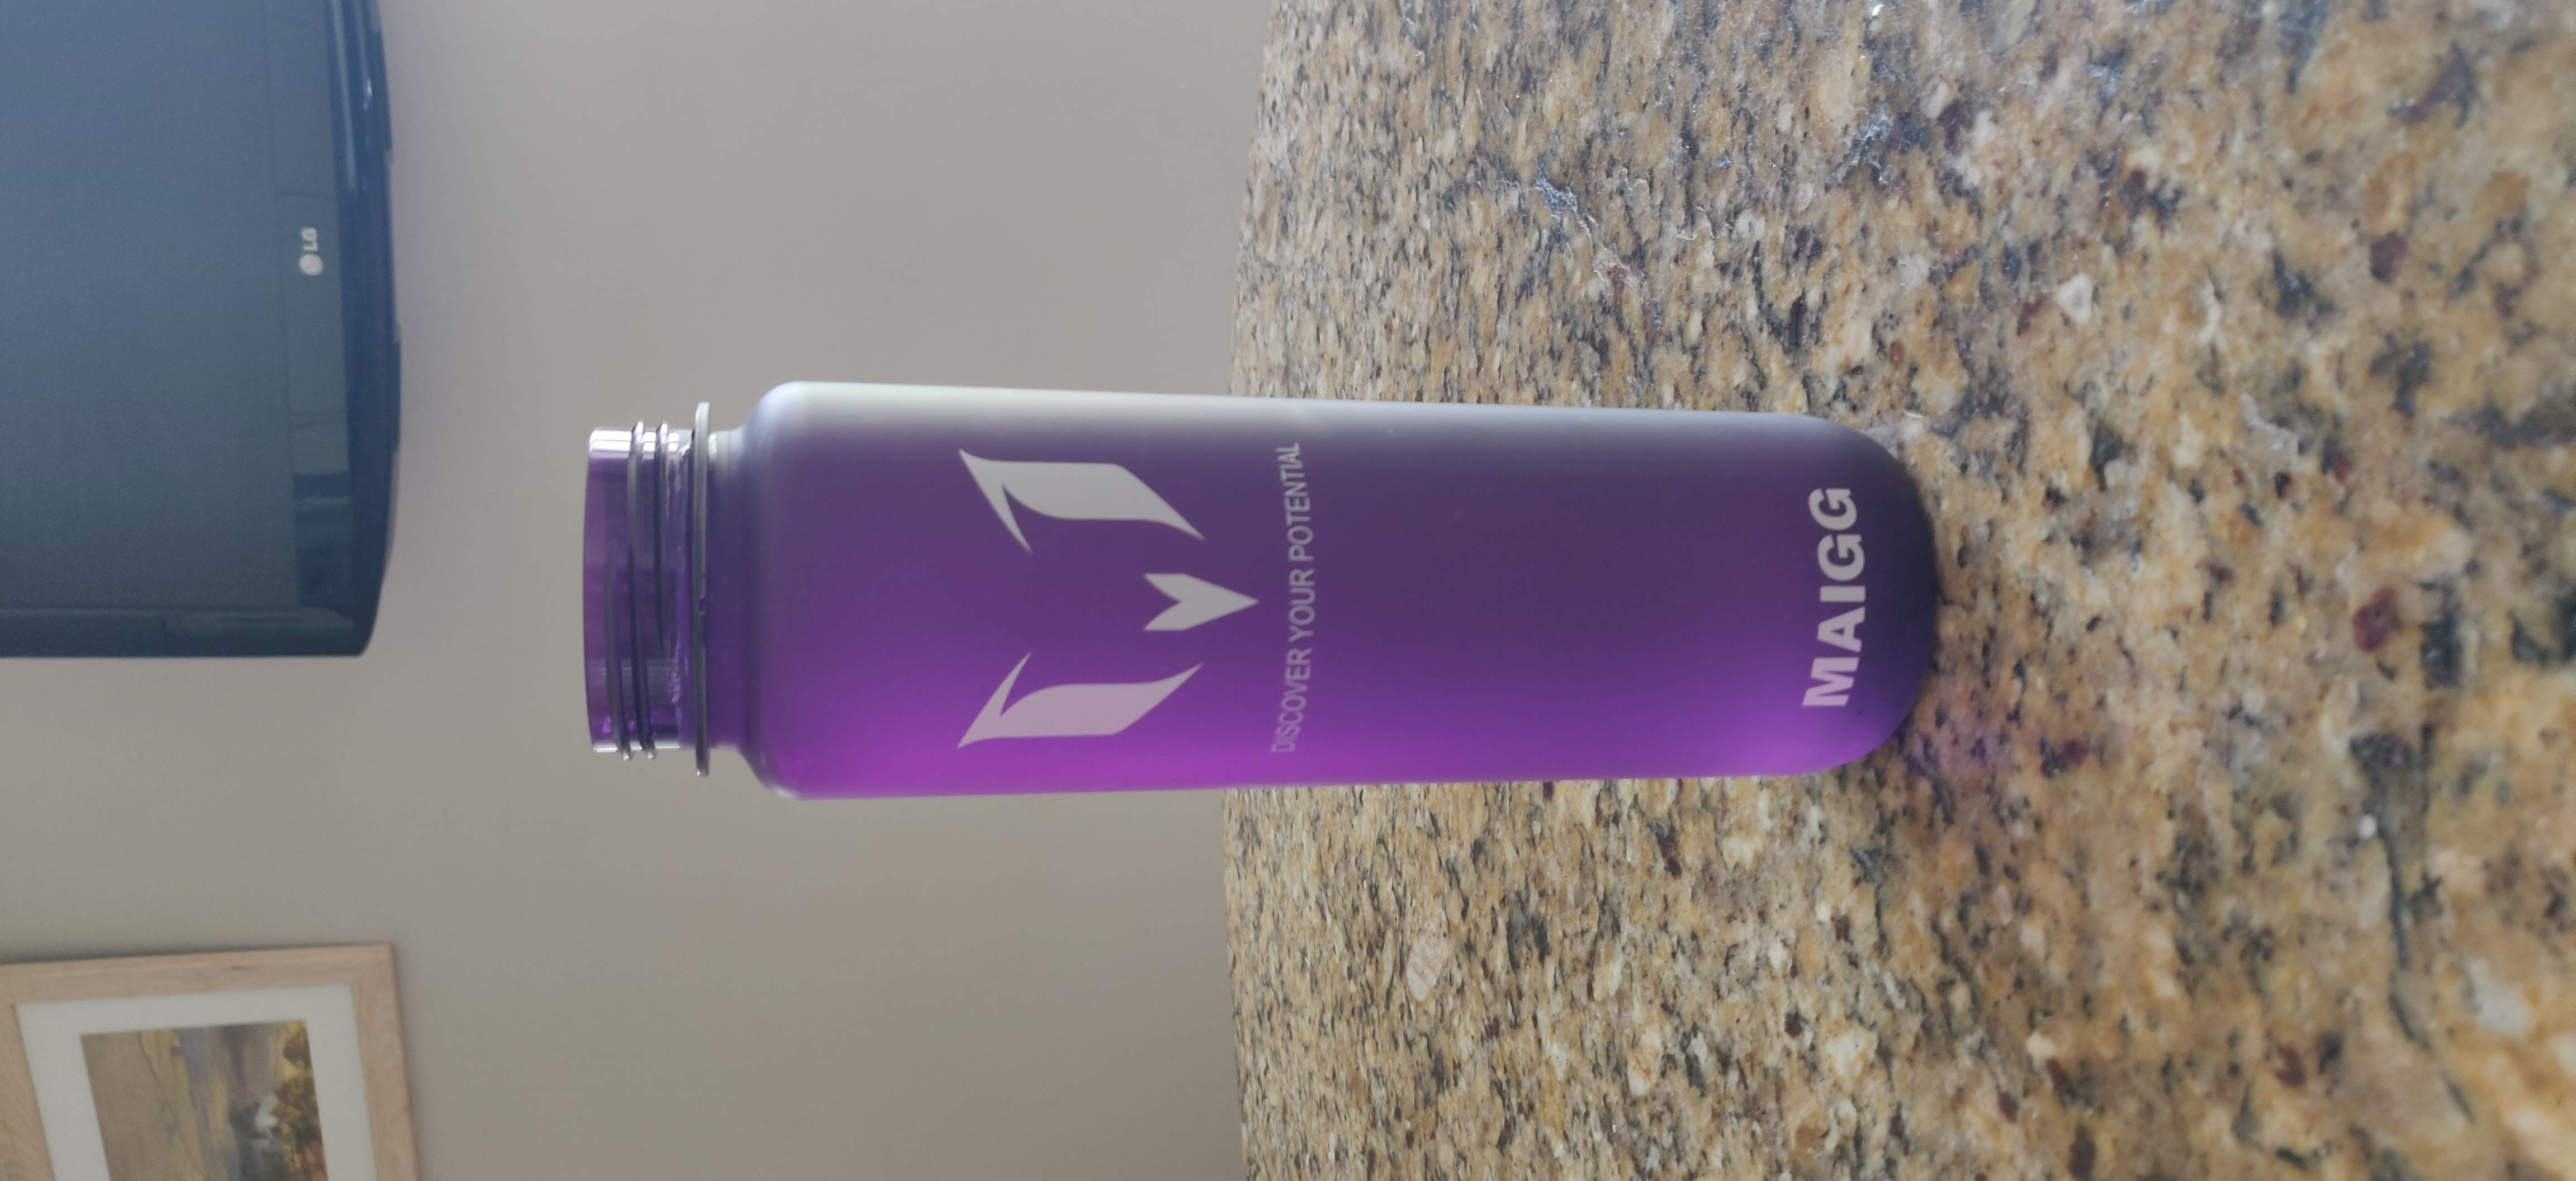
\includegraphics[width=\textwidth]{reference/bottle_face_on.jpg}
        \caption{Front face of the bottle showing the logo and writing.}
        \label{fig:face}
    \end{minipage}
    \hfill
    \begin{minipage}[b]{0.3\textwidth}
        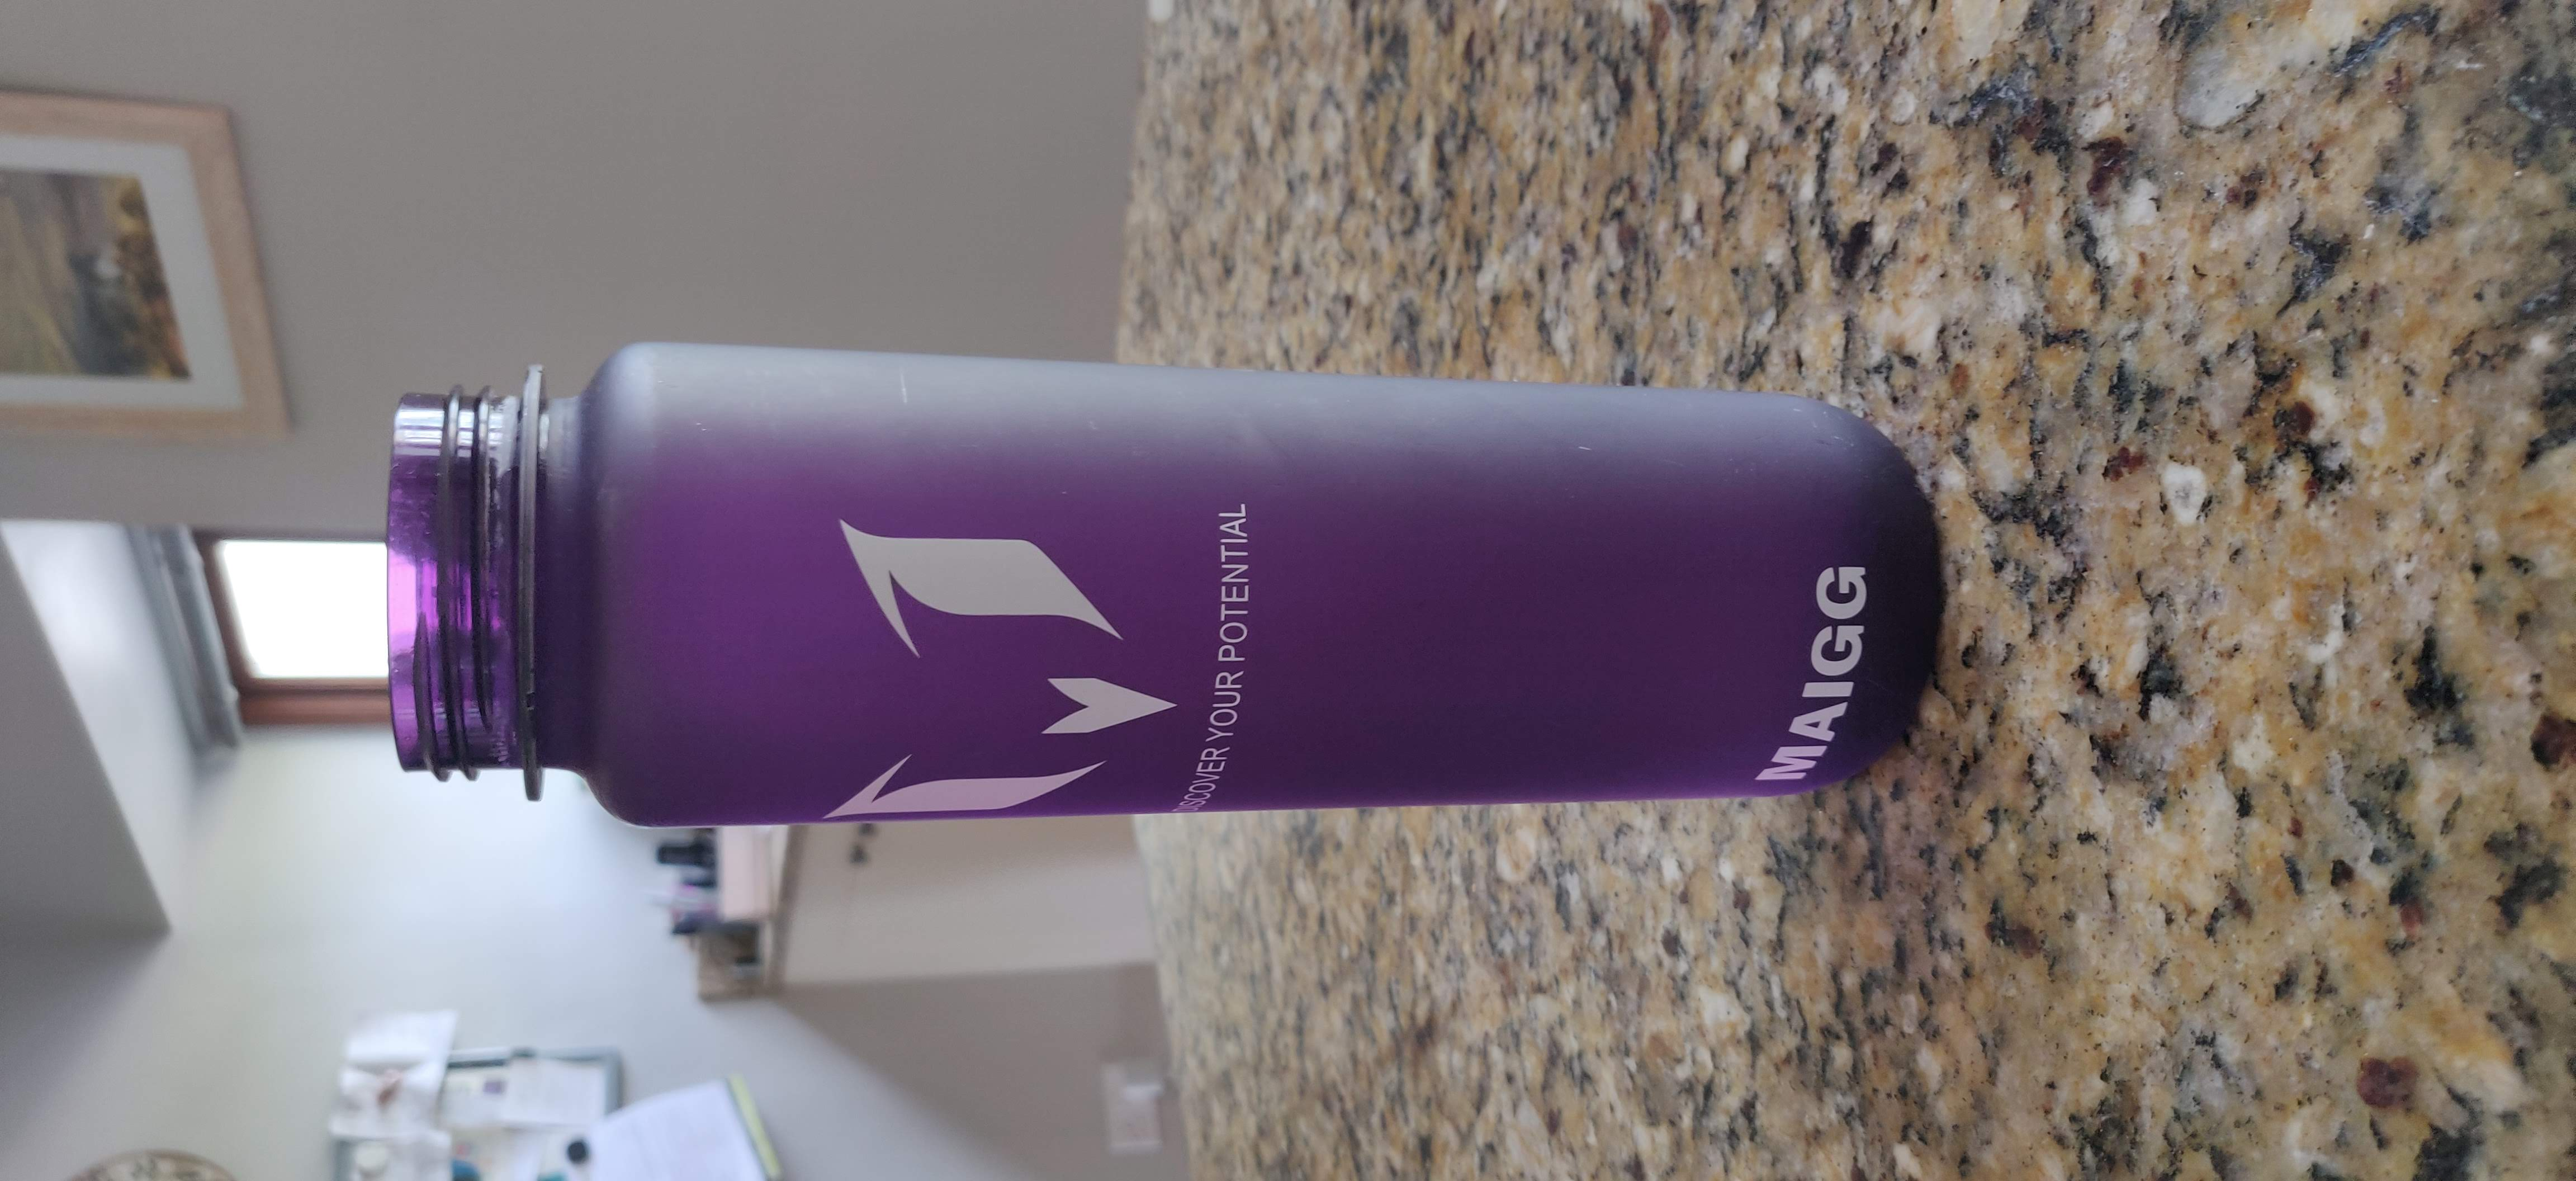
\includegraphics[width=\textwidth]{reference/bottle_right.jpg}
        \caption{Right side of the bottle showing diffuse reflection.}
        \label{fig:right}
    \end{minipage}
\end{figure}

The object chosen for this assignment is a water bottle made my MAIGG. I chose to remove the cap and only focus on the body of the bottle to simplify the object, as the cap was much more complicated.

The bottle is predominantly a long, thin cylinder. At both the top and bottom of the bottle, the shape curves in to give the bottle a nicer look and to avoid sharp edges. At the very top of the bottle is a threaded section that is used to attach the lid of the bottle (see Figure \ref{fig:thread}). Just below the threading is a rim that stops the cap being screwed on too far.

To implement this in Renderman, I first started with a basic cylinder that wraps the full 360 degrees. I originally started trying to make various sizes of cylinders on top of each other to create the narrower shapes and the threading section, which I would then displace to blend between each, however I realised the entire shape could all be achieved with a single displacement shader and thought it was more impressive going from a single cylinder to the final bottle shape. I talk more about this displacement shader in Section \ref{section:tex_displace}.

\subsection{Colour and Material}

When the bottle has a stronger light behind it, the colour is much darker but the main colour is a dull purple. The surface of the bottle is smooth but cloudy making the reflections not very clear, showing only simple colours rather than reflected objects (see Figures \ref{fig:face} \& \ref{fig:right}). The bottle is made of a cloudy plastic that only lets a low level of light through, but there is still some refraction visible.

In Renderman, I chose to do all the shader work using PxrLayers. For each bottle, the base layer was the basic colour of the bottle (e.g. red, blue, or purple). These layers were then mixed using PxrLayerMixer, and the output colour was used in my Bxdf. The Bxdf was where I implemented the cloudy plastic, reflections, and refractions. I made the bottle have a semi-rough diffuse setting to give the same reflections as the reference, and used the glass settings to make the material behave as a rough plastic with poor reflections but still some refraction.

\subsection{Textures and Displacement} \label{section:tex_displace}

\begin{figure}[ht]
    \centering
    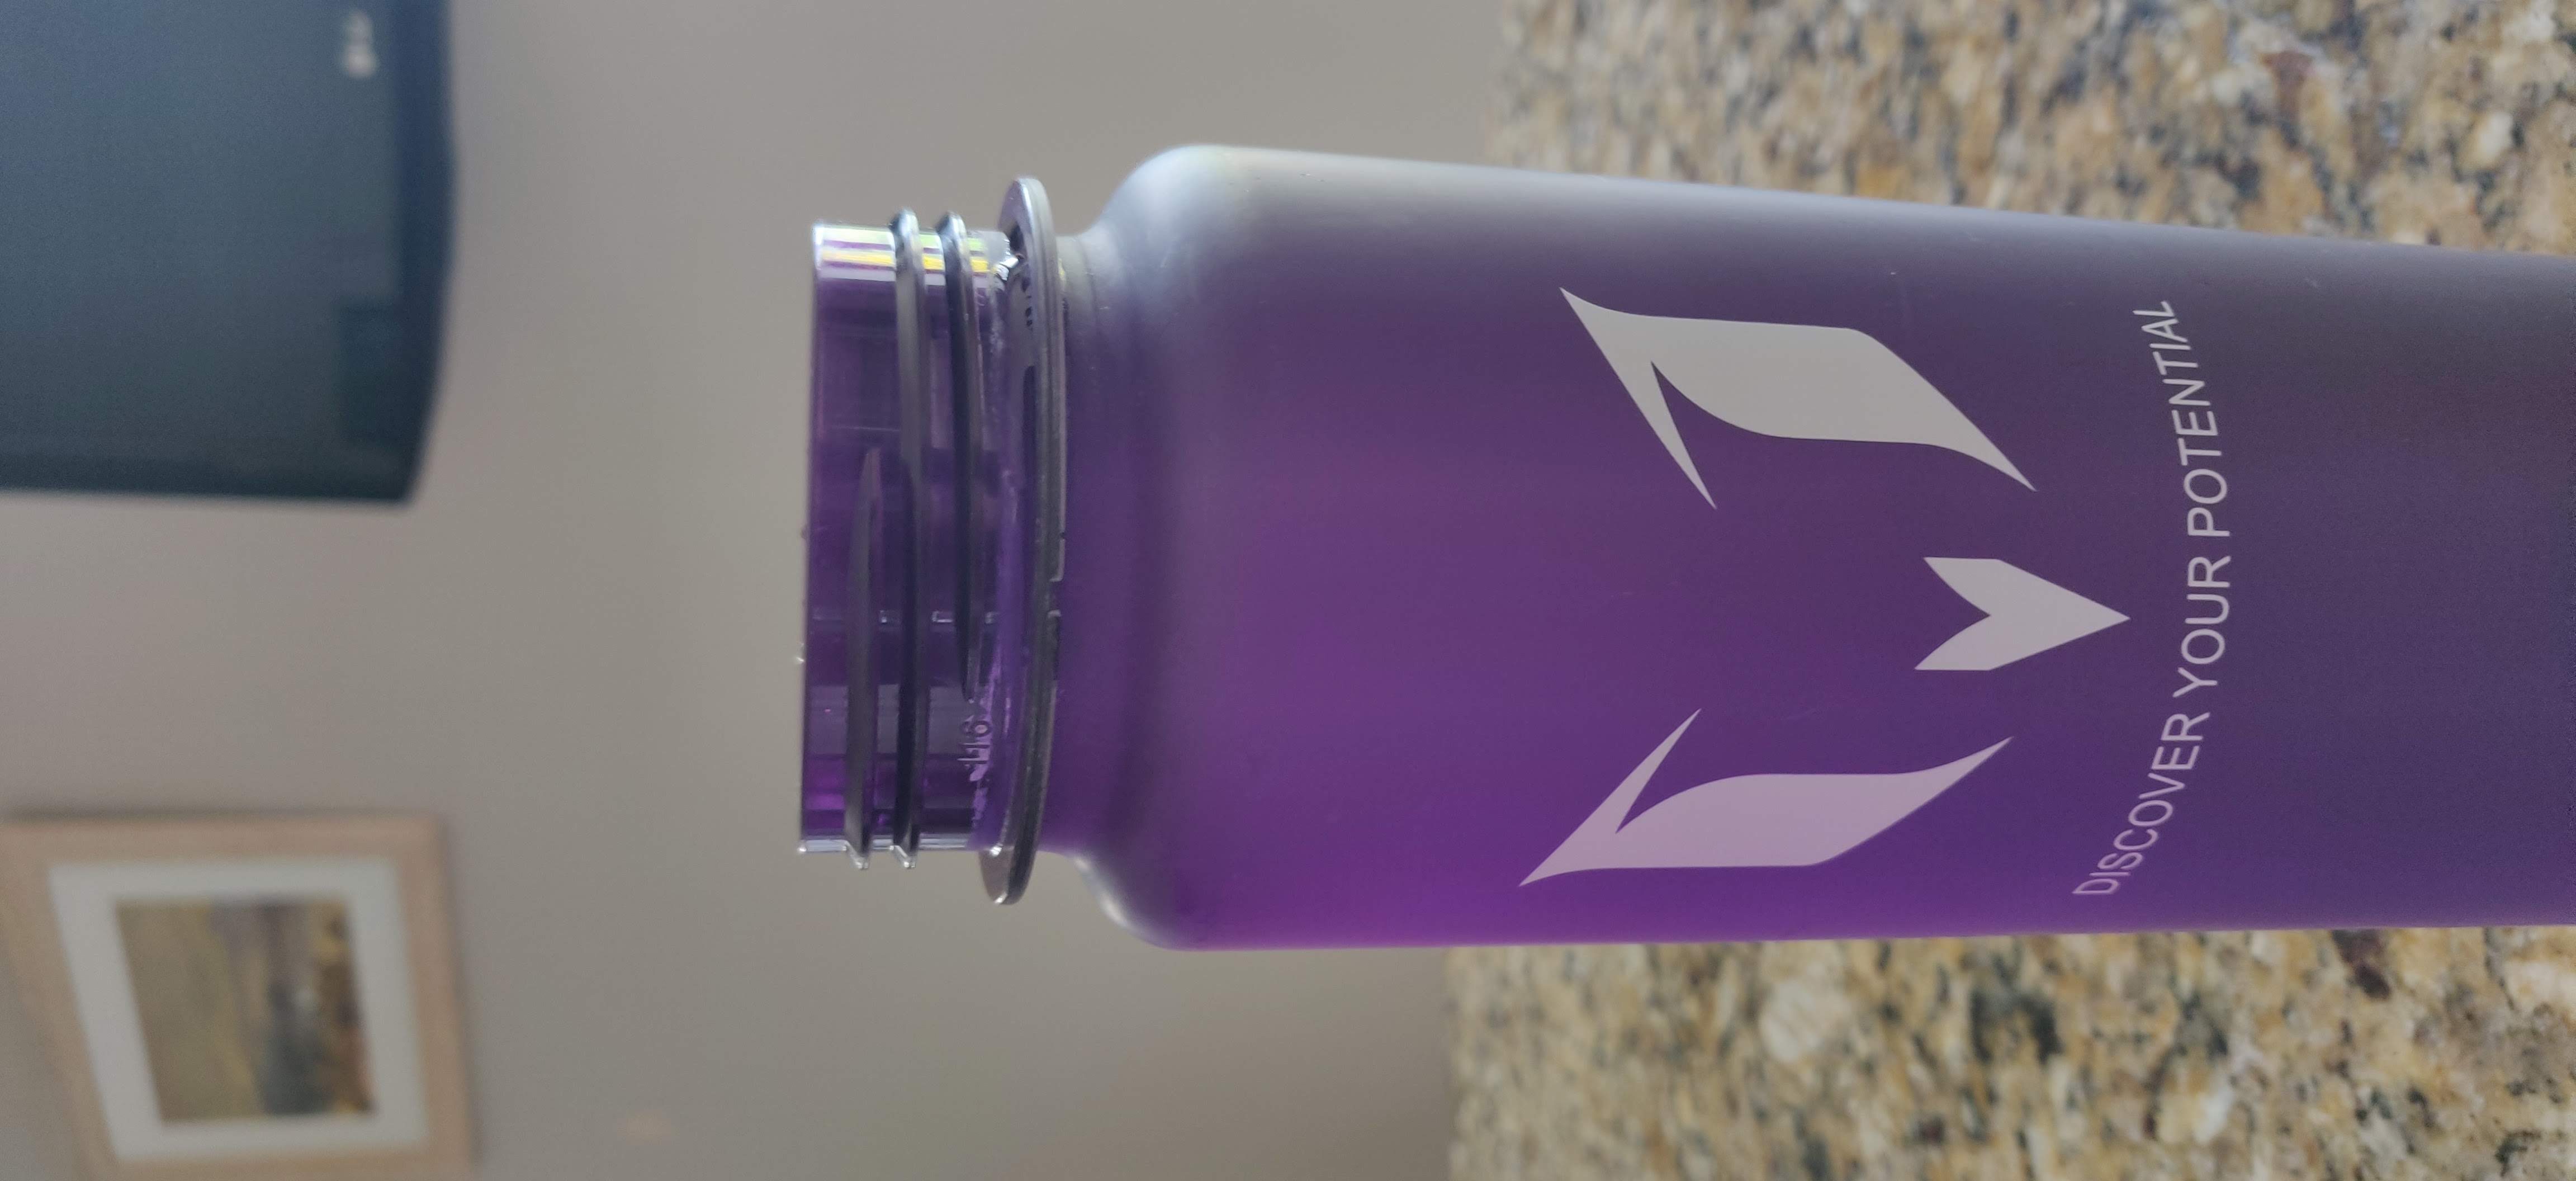
\includegraphics[width=0.5\textwidth]{reference/bottle_thread.jpg}
    \caption{Threading at the top of the bottle used to connect cap.}
    \label{fig:thread}
\end{figure}

On the front of the bottle is a logo and two lines of text. The logo is a minimalistic, single colour sparrow. The first line of text, lies right beneath the logo and reads ``DISCOVER YOUR POTENTIAL'' in a small, narrow font, with the second line of text reading ``MAIGG'' in a larger, bold font. As mentioned in Section \ref{section:model}, the bottle shape curves out, then is flat, then curves back in, and finally, a threaded cap attachment is at the top.

A texture was used for the logo and text when implementing the bottle in Renderman. I thought about making a shader that made the logo using maths but felt it would be a better use of my time to focus elsewhere. Instead, I opened Figure \ref{fig:face} in a photo editor and drew a 4k version on top. This texture was then scaled appropriately and converted to .tx using txmake. This texture was then used in a PxrTexture and combined with the other layers in the PxrLayerMixer. 

The displacement shader was responsible for getting the shape of the bottle. The bottom and top curve were made using the subtraction of two smooth steps at each curve, and then square-rooted to give a curved shape. The notch below the threading was the subtraction of two steps instead, that created the sharp step out, but not as far as the displacement of the curves. Finally, the thread used the same stepping as the notch but the value used in the step function was based on the value of u, giving a spiral effect. This was repeated twice to give two rotations of threading.

\subsection{Variation and Wear}

As I have had the bottle for a few years now, naturally there were a few scratches, scuffs, and dirt patches on the bottle. The colour of the bottle is also not uniform all over, with various patches slightly faded or darker than the base colour. The logo and text has fortunately had no scratches so far and still looks as it did when the bottle was first purchased.

Therefore, in Renderman, I needed to firstly add some colour variation to each of my bottles. This was achieved using a custom shader that based on Perlin noise, created large patches of a slightly different colour to the base colour. This worked by taking the point, scaling it to create larger patches, then mixing the base colour with a slightly duller colour. This was then combined in the PxrLayerMixer.

For the dirt and wear, I used one custom shader that worked in a similar way to the discolour shader. The dirt layer was scaled in x to create longer strands of dirt and stains that looked more realistic than lots of blotches. The wear was achieved by applying two layers of the dirt shader, one with a low frequency for the areas that were scuffed, and the second with high frequency and scaled in y to create vertical scratches and variation in these areas.

\subsection{Lighting and Environment}

The lighting in my references is quite dull with no strong shadows or direct light. Instead, the light is quite diffuse and due to it being an overcast day, the lighting was quite grey. The bottle was photographed on granite in a kitchen, giving slight reflections of the bottle.

Even though the bottle was photographed on granite in a kitchen, I couldn't find a suitable HDR image of a kitchen and felt making my own HDR would be too time consuming, so I opted to use one I found online of a bird lookout as I felt the sky colour was similar, and it wouldn't be out of place to see a bottle in this location. The HDR was used in Renderman by importing it into a PxrDomeLight, rotating it to be the right orientation and position.

I chose to place multiple bottles in the first scene to show multiple versions of the wear and to show how different colours of the bottle would look. However, instead of creating a ground plane like the granite in the reference photos, I opted to use the wood shader from one of the lectures so I could focus more on other areas. The Bxdf for the table used the clear coat features to make the table look as though it had a layer of varnish on top, giving the wood some reflection and colour variation as parts in direct light would appear to be more amber in colour, just like how varnished wood looks in real life.

\subsection{Camera Effects and Post-Processing}

In the references, the only perceived camera effect is depth of field. This blurs the background slightly as the camera is focused on the foreground object. There are no other effects as the lighting is dull and the object and camera are stationary.

Therefore, in Renderman, I used the depth of field settings to make the main bottle in focus, with the background out of focus to the point where you can't make out much of the environment and the other bottles are slightly out of focus.

\begin{figure}[ht]
    \centering
    \begin{minipage}[b]{0.48\textwidth}
        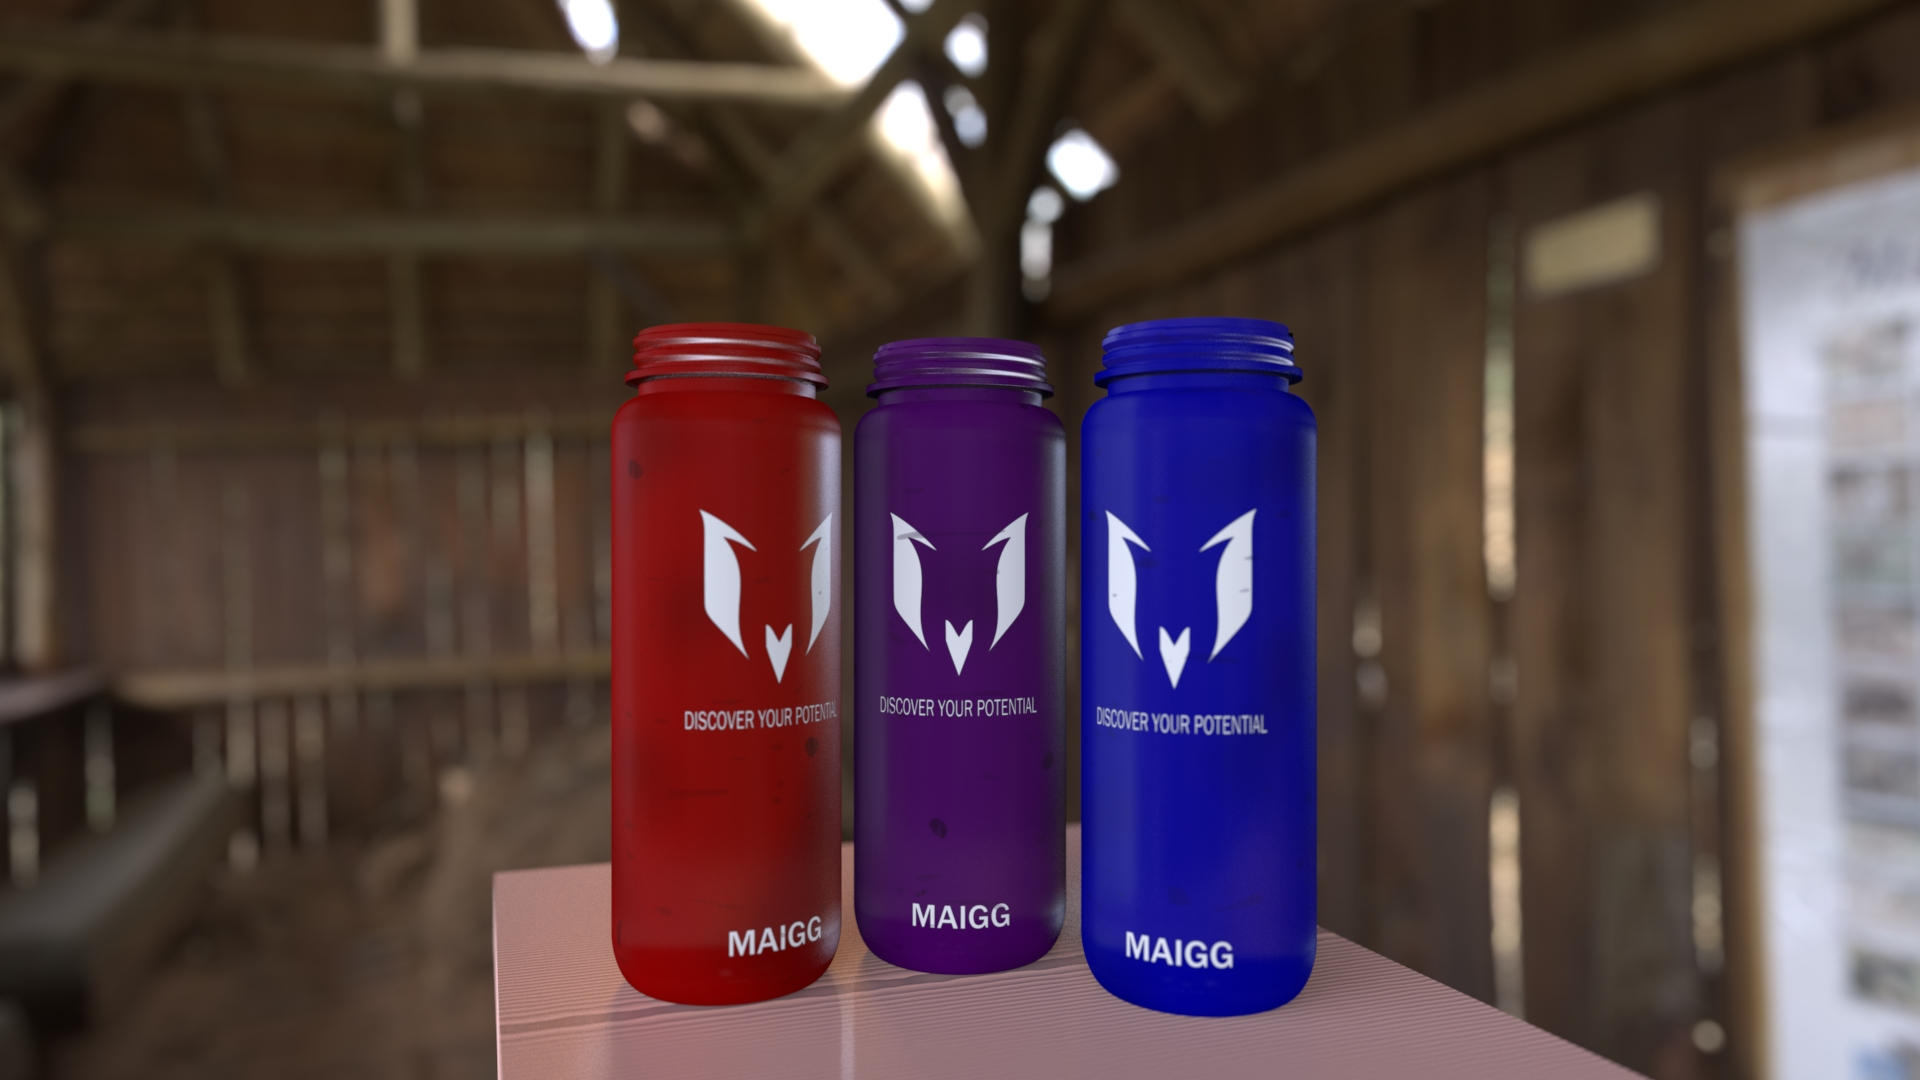
\includegraphics[width=\textwidth]{render/bottle.jpg}
        \caption{The main render, showing three coloured bottles.}
        \label{fig:render}
    \end{minipage}
    \hfill
    \begin{minipage}[b]{0.48\textwidth}
        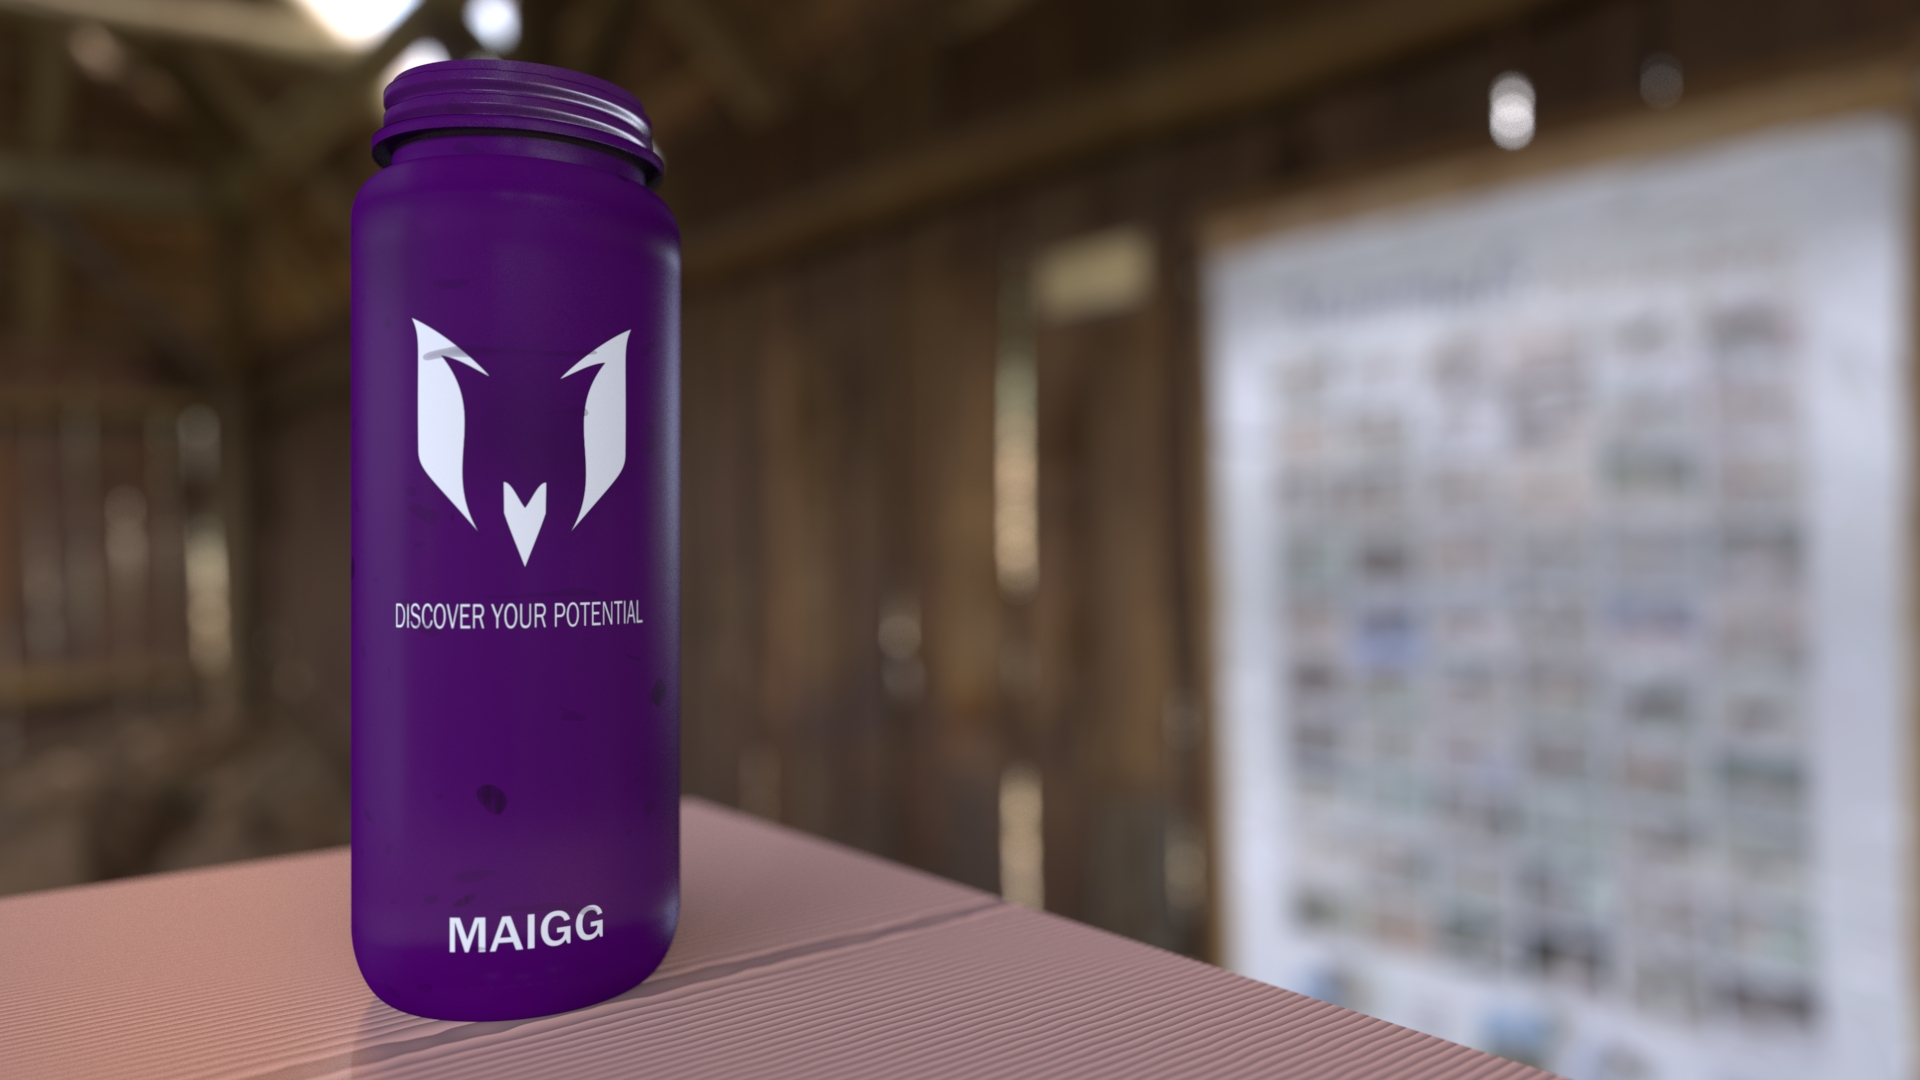
\includegraphics[width=\textwidth]{render/bottle_alternate.jpg}
        \caption{An alternate render showing one bottle at a different position.}
        \label{fig:render_alt}
    \end{minipage}
\end{figure}

\end{document}
